\chapter{State-of-the-art}
\label{chapter:stateofart}

\section{Overview}
\label{section:overview}
A detailed description is provided in this section concerning the state of the art technologies existing nowadays in the market.  The main integration technologies available today are based on Web technologies, namely HTTP, XML, JSON, Web Services using either SOA or REST architectural styles, with Web Services and REST on HTTP. This section also gives information about new tools such as HTTP/2 and WebSocket technologies that will be used in our solution.
%%%%%%%%%%%%%%%%%%%%%%%%%%%%%%%%%%%%%%%%%%%%%%%%%%%%%%%%%%%%%%%%%%%%%%%%
\section{Web Services}
\label{section:webservices}

Web services allow you to use two different machines or two different pieces of code that talk each other. Two different applications can talk to each other over the network. They can call methods of each other over the network by using web service technology. The other advantage of using web services is that actually it is a standard technology because it is not really specific to Java or any other language. You can write web services using all other technologies. For example you can write a web service with Java, .Net, Python, C++ or others. The best part of web service standard what is called as Interoperability that  is a property of a product or system, whose interfaces are completely understood, to work with other products or systems, present or future, without any restricted access or implementation\citep{thesis:state1}.

\begin{figure}[!htb]
  \centering
  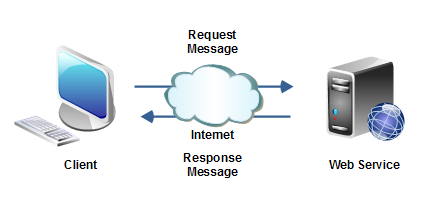
\includegraphics[width=0.5\textwidth]{Figures/web-service-message-formats-1.png}
  \caption[Simple Web Service Architecture.]{Simple Web Service Architecture.}
  \label{fig:webservice}
\end{figure}

For example let’s say you have written web service in Java, let’s say you have another web service that written in .Net so what the web service technology allows you to do is, Java can call .Net web service and .Net web service can also call Java web service and it just doesn’t have to be web service because it can be an application. Let’s say you have another application written in C++, so you can actually have C++ app that call Java web service or .Net web service. You can actually have different applications written in different
technologies that communicate with each other during execution time and they can call each other. This actually let us to do that you can actually pick and choose technologies that you want to use let’s say you have set of business web services that are implemented in .Net and your Java application can use them.

Web Services are exposed to the Internet for programmatic access. They are online APIs that you can call from your code. When you want to call any API that written by someone else to your Java code, you basically add jar or classes to your class path and executions are done inside of machine or single environment. In the case of web services however you have different pieces of code deployed over different machines and they call methods of each other over the network. For example, you must have seen that different apps or games, which can post to your Facebook wall even these games, not designed by Facebook. So you ask that how they can do that or how they can post to a wall of completely different system or application. Basically they do this by calling online APIs. Companies like Facebook or Twitter publish web services that let other developers call them from their code, so other application developers can actually write code to consume these services and they can post things on Facebook or Twitter. They can read or access data from Facebook or Twitter using the APIs of the web services that Facebook or Twitter has provided.

Web services are similar to web pages. For example Twitter has web side URl called as “www.twitter.com”  when you access this URl on your browser you get an HTML response that let you read and write tweets. They have HTML elements for data and also CSS files for styling, this is because web pages that you see are made for human conception. They know that there is actually human is behind of browser on a laptop or devices who was reading these tweets, so they want to make sure about its format properly, thats way it is easy to access and read. Twitter has also other URl as “api.twitter.com” that does a lot of same things as “www.twitter.com” does, but it behaves a bit differently for instance this API gives you response which doesn’t have HTML or CSS code. It contains data but it is XML or JSON format and there are specific URls for different operations this is what the developers can use from their code to read or write to twitter, so this data is actually very easy for parsing and converting then using in their objects and their code for developers. In this case there is no need to have HTML and CSS files.

There are primarily two different types of web services. One of these types called as  Simple Object Access Protocol (SOAP) web service and another type called as REpresentational State Transfer(REST) web service. SOAP is older of these two and REST is newer entry to web services world, but both of them are used popular. Next section will be focusing on SOAP and REST web services.

%%%%%%%%%%%%%%%%%%%%%%%%%%%%%%%%%%%%%%%%%%%%%%%%%%%%%%%%%%%%%%%%%%%%%%%%
\section{SOAP Web Services}
\label{section:soa}

Simple Object Access Protocol, or SOAP as it was the first attempt to standardize a web service interface. It is based on sending an XML message to a service, in a specific XML format, and receiving an XML response in another specific format. The message can be sent across different transports, including HTTP, FTP (File transfer Protocol), SMTP (Simple Mail Transfer Protocol) and more\citep{thesis:state2}. The specification does not dictate the transport over which the message should be sent, but most implementations send the XML message over HTTP.

Now it will be explained shortly SOAP web service by an example. Let’s start an example with Java application. Let’s say you have implementation class and you want to share this implementation class with other developer projects. How you would share this with a consumer class. The best way to share this implementation class would be to contract it with an interface and other consumers would consume this class through this interface. They would call implementation through interface so they get contract and they get the methods, arguments, written types through interface. They actually call the methods of implementation class, so how this works in case of web service, let’s say you have web service implementation and you want to share details of this web service to consumers. Is it works with an interface? Probably it will not work because as discussed before you don’t know what technology is consuming it. It might be .Net application or C++ application, so if you have a java web service you might want to give some kind of information that its consumer respects to that technology and that can actually consume. Let’s say consumer is .Net and if you give this .Net application a Java interface then most probably it will not work because they are different technologies, so the technology that you are going to share with web service consumer has to be technology independent. It should be something that any application or any technology can understand so creators of SOAP web service talked about that problem and what to give format understandable by all technology with all consumers and decided with XML. So what you do is in case of web service, you actually share that contract as an XML document. This XML document is actually called as WSDL(Web Services Description Language)\citep{thesis:state3}.

WSDL (a set of conventions on XML usage) document contains the contract to web service and so that’s are the things you have to do when you create the web service and you share WSDL document of that web service to the consumers, so this is not something you would have to do it manually. You would do it manually but there are tools which generate WSDL for the web service. There is a stub generator for every language to create that WSDL document. It is something that you need to share this WSDL to consumers and it is a XML document, so it respective whatever application because applications such as .Net, C++ or Java can all parse this XML\citep{thesis:state4} and get to know about service information and typically the content of this WSDL is kind of similar to an interface content. It has operations, arguments and types  to return that consumer applications will have idea what to call and how to call.

\begin{figure}[!htb]
  \centering
  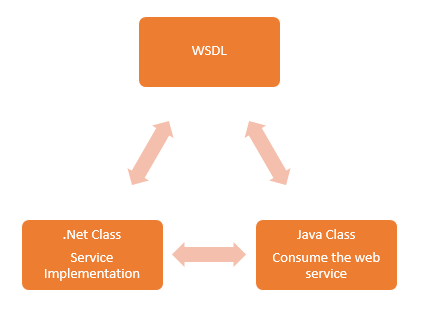
\includegraphics[width=0.5\textwidth]{Figures/WSDL.png}
  \caption[WSDL (Web Services Description Language).]{WSDL (Web Services Description Language).}
  \label{fig:wsdl}
\end{figure}

The new question is that how this exchange happens, how you actually send this information, let’s say you have a method in your java application and input argument is a string so you have a java string with you and you need to send to web service and let’s say output return type is a list, so how you get this information because that could be .Net application and string in Java obviously different from string in .Net. How do you exchange this between client app and web service?  When you exchange information input argument or return type, you need to exchange it in the format that all different technologies can understand what you are passing and it should be able to send return type back in language that all these technologies can understand. Again this format is XML. When you are sending any information across the network from a client to the web services and
return type back to the client, the data has to be in XML format. You are not really sending Java string or a list. So it has to be language natural format which is XML. There is specification about how you need to send all these different input type and output argument basically any type needs to be send specific XML format. It is a protocol that is a way in which both sender and receiver use and this XML is called SOAP(Simple Object Access Protocol). It is a way in which these different technologies can access objects can access data it supposedly simple so that a part of the name is called simple object access protocol. So with this protocol all different technologies written in different languages can kind of understand what they all taking about.

\begin{figure}[!htb]
  \centering
  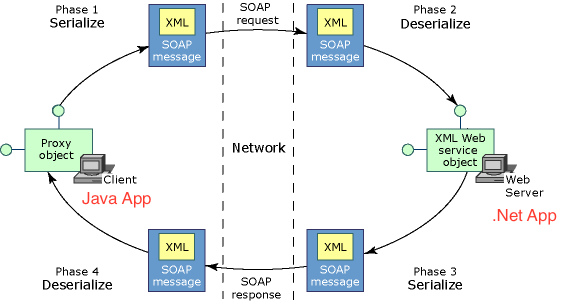
\includegraphics[width=0.9\textwidth]{Figures/soap.png}
  \caption[SOAP (Simple Object Access Protocol).]{SOAP (Simple Object Access Protocol).}
  \label{fig:wsdl}
\end{figure}

Now you know what is the mechanism, you know what need to be send and you know how to send which is using SOAP protocol but who does conversion? So for example you have your string object or complex object, so how do you convert it from Java object to a SOAP message? The conversion is actually done with intermedia class so this class takes care of converting all your objects into a SOAP message. The whole method calls itself is actually done by SEI(Service Endpoint Interface)\citep{thesis:state5}. The SEI access interface to your web service endpoint so you have an interface at your client app to the service endpoint which translate all web service call to a SOAP message and then it makes sure that the other things is able to understand this message. So you don’t have to write this class and all the conversion ourself. You can have it automatically generated for you. When you are making a web service call you don’t worry about where the web service is. When you need to call, all you need to do is have this endpoint interface and good thing about this service endpoint that you can actually have an interface that specific to what you are developing. When you have a java application you will have a specific SEI for java application and it knows to convert Java objects to SOAP message. Let’s say your .Net application calling the same web service so you will have SEI for .NET that know to convert .Net objects to SOAP message.

%%%%%%%%%%%%%%%%%%%%%%%%%%%%%%%%%%%%%%%%%%%%%%%%%%%%%%%%%%%%%%%%%%%%%%%%
\section{REST Web Services}
\label{section:rest}
REST (Representational State Transfer) was created in 2000 by Roy Fielding\citep{thesis:state5_1}. Developed in an academic environment, this protocol embraces the philosophy of the open Web. Instead of using XML to make a request, REST relies on a simple URL in many cases. In some situations you must provide additional information in special ways, but most Web services using REST rely exclusively on obtaining the needed information using the URL approach. REST can use four different HTTP 1.1 verbs (GET, POST, PUT, and DELETE) to perform tasks.

Resources are the fundamental building blocks of web-based systems. A resource is anything to be exposed to the Web,
from a document or video clip to a business processor device. A URI uniquely identifies a web resource, and at the same time makes it addressable, or capable of being manipulated using an application protocol such as HTTP. The relationship between URIs and resources is many-to-one\citep{thesis:state5_2}. A URI identifies only one resource, but a resource can have more than one URI. That is, a resource can be identified in more than one way, much as humans can have multiple email addresses or telephone numbers. This fits with your need to identify real world resources in more than one way. Everything in REST web services has URl is unique and standard. For example Facebook, when you open an account on Facebook, you will get a profile page that obivously dynamically generated pages, so whenever there is a new profile, it basically the same page which does same processing but render different content depending on profile that you are watching. In REST web services you need to think of resources and create unique urls for them. For example you are creating weathercast application and you want to get weather for different cities of Portugal, so your URl needs to be unique for each city as in table \ref{tab:urlexample}.

\begin{table}[!htb]
  \renewcommand{\arraystretch}{1.2} % more space between rows
  \centering
  \begin{tabular}{lccc}
    \toprule
    URl & Description  \\
    \midrule
    http://weatherapp.com/city/Lisbon &  Unique URl for Lisbon city\\
    http://weatherapp.com/city/Porto & Unique URl for Porto city\\
    http://weatherapp.com/city/Algarve & Unique URl for Algarve city\\
    \bottomrule
  \end{tabular}
  \caption[URl Example.]{URl Example.}
  \label{tab:urlexample}
\end{table}

In REST web services, with same unique URl that can be done different actions, for example if you are administrator of weathercast application and you want to get data of Lisbon city or if you want to update data of Lisbon city or deleting data of Lisbon city you can use the same unique URl for all these methods using HTTP methods. Only a single concrete URI, a single URI template, and four HTTP verbs. In fact, it’s so compact that can be provided an overview in just a few lines, as shown in Table \ref{tab:aeroCoeff}.

\begin{table}[!htb]
  \renewcommand{\arraystretch}{1.2} % more space between rows
  \centering
  \begin{tabular}{lccc}
    \toprule
    Verb           & URI or template & Use  \\
    \midrule
    POST           & /city & Create a new city\\
    GET            & /city/{cityName} & Request the data of city specified by the URI.\\
    PUT            & /city/{cityName} & Update an city data at the given URI with new information.\\
    DELETE         & /city/{cityName} & Logically remove the city identified by the given URI.\\
    \bottomrule
  \end{tabular}
  \caption[HTTP Methods.]{HTTP Methods.}
  \label{tab:aeroCoeff}
\end{table}

\begin{figure}[!htb]
  \centering
  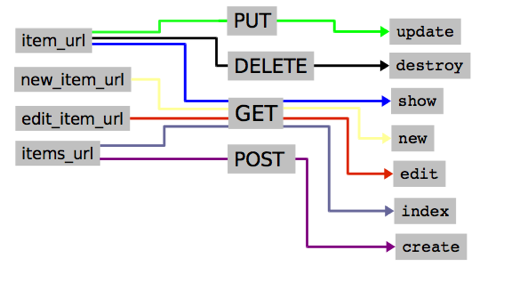
\includegraphics[width=0.8\textwidth]{Figures/rest.png}
  \caption[REST URIs and HTTP methods.]{REST URIs and HTTP methods.}
  \label{fig:rest}
\end{figure}

You've seen the requests so far, and understood what resource URIs and HTTP methods. You make request to resource URIs with using HTTP methods. Let's switch to responses now. After making request, RESTful web service will be responded. It is important format of response because client needs to write code to handle that response. if that were a web application, the response would be HTML page with styling formatting. When it comes RESTful Web service you don't need all this styling because it can be basically XML or JSON. Following section will give detailed information about XML or JSON.
% ----------------------------------------------------------------------
\section{Serialization formats (XML, JSON and Binary)}
\label{section:xml}
The contents of messages in distrubuted systems need to be serialized to be sent over the channel and the format to do so (such as XML or JSON). A schema is used to transform the internal data structures into serial messages and vice-versa. The serialization formats used in the Web (e.g., XML, JSON) are text-based and thus verbose and costly in communications. Technologies have been developed to compress text-based documents\citep{thesis:state5_3}, such as EXI (Efficient XML Interchange), BSON and others \citep{thesis:state5_4}. However, these are compression technologies, which need text parsing after decompression.
\begin{lstlisting}[caption=Example Person Object Class, label=lst:person]
  public class Person {
    public String name;
    public int age;
    public String eyeColor;
    }

  Person p = new Person();
  p.name = "Peter";
  p.age = 34;
  p.eyeColor = "blue";
\end{lstlisting}

XML, which maintained the text markup style of HTML, made computer based clients easier and, together with HTTP, became the cornerstone of Web Services technologies. This evolutionary transition is perfectly understandable in market and standardization terms, but still constitutes a mismatch towards both humans and applications. XML is text based and support schemas. XML retains the look and feel of HTML, with text markup based on start and end tags as seen example in in Listing ~\ref{lst:xmlperson} of in Listing ~\ref{lst:person} Person Object. XML has generalized HTML, separating data from formatting and introducing self-description with a schema, but retained much of its look and feel, still with a data document nature (just data, instead of a more complete service nature, by including code) and text with markup (lacks native binary support). There are technologies such as  EXI, the binary XML format, which offers compression at less cost than using Gzip, and save processing otherwise needed to decompress compressed XML\citep{thesis:state9}.

\begin{lstlisting}[caption=JSON presentation of Person object, label=lst:xmlperson]
  <Person>
    <name>Peter</name>
    <age>34</age>
    <eyeColor>blue</eyeColor>
  </Person>
\end{lstlisting}
JSON is much more populer than XML\citep{thesis:state6}, as a simpler alternative to XML because it is more compact especially you have large amount of data and also when client is browser which is piece of javascript code running on browser so sending response data in JSON can be easily parsed by client. JSON delimits data with syntax tokens, with a simple grammar that bears some similarity with data structures in C-like languages as seen example in in Listing ~\ref{lst:jsonperson} of in Listing ~\ref{lst:person} Person Object. XML has targeted flexibility and generality, whereas JSON has emphasized simplicity, which is after all the secret of its popularity. There is also BSON, the binary JSON format devised by 10gen and used in their MongoDB NoSQL database, instead of JSON \citep{thesis:state8}. As described before these are compression technologies, which need text parsing after decompression.

\begin{lstlisting}[caption=JSON presentation of Person object, label=lst:jsonperson]
  {
  "Person":
    {
    "name": "Peter",
    "age": "34",
    "eyeColor": "blue"
    }
  }
\end{lstlisting}
In spite of the differences, both suffer from drawbacks and limitations:

They are text based, which means inefficient parsing and data traversal where all characters of a component need to be parsed to reach the next one, high memory consumption, relevant message transmission times and poor support for binary data. The serialization format should be as close as possible to the data structure to minimize the conversion effort in serialization and deserialization. Text can be thought as human readable and therefore advantageous over binary, but this is true only for very simple documents, especially when using XML. Binary compression mechanisms exist \citep{thesis:state5_3}\citep{thesis:state5_4}, but this does not reduce the parsing time, since text need to be recovered. It would be better to follow the old example of programming languages, by using a source format for humans, a binary format for computers and a compiler to synchronize them.\citep{thesis:state6}

% ----------------------------------------------------------------------
\section{HTTP/2}
\label{section:http2}
HTTP/2 is the second major version of the HTTP network protocol used by the World Wide Web. HTTP/2 will make our applications faster, simpler, and more powerful. The primary goals for HTTP/2 are to reduce latency by enabling full request and response multiplexing, minimize protocol overhead via efficient compression of HTTP header fields, and add support for request prioritization and server push\citep{thesis:state10}.

The first important thing to notice about HTTP/2 is that it is not a replacement for all of HTTP. The verbs, status codes and most of the headers will remain the same as today. HTTP/2 is about becoming more efficient in the way data is being transferred on the wire\citep{thesis:state11}.

HTTP/2 breaks down the HTTP protocol communication into an exchange of binary-encoded frames, which are then mapped to messages that belong to a particular stream, and all of which are multiplexed within a single TCP connection. HTTP/2 communication is split into smaller messages and frames, each of which is encoded in binary format. This is the foundation that enables all other features and performance optimizations provided by the HTTP/2 protocol.

HTTP/2 uses header compression to reduce overhead. Typical header sizes of 1KB are common mainly because of the cookies that all have to be accepted for a smooth user experience. Transferring 1KB can take several network round trips just to exchange headers, and those headers are being re-sent every time because of the stateless nature of HTTP

HTTP/2 Server Push allows servers to proactively send responses into client caches. In a typical HTTP workflow, the browser requests a page, the server sends the HTML in the response, and then needs to wait for the browser to parse the response and issue additional requests to fetch the additional embedded assets (JavaScript, CSS, etc.). Server push allows the server to speculatively start sending resources to the client. Here, the browser does not have to parse the HTML page and find out which other resources to load; instead the server can start sending them immediately.
% ----------------------------------------------------------------------
\section{Web Sockets}
\label{section:websockets}

WebSockets\citep{Ontology:matching} are a relatively new technology which promises to make websites more reactive by allowing lower latency interaction between users and the server. WebSockets circumvent some of the limitations of HTTP which removes this restriction, adds binary support and increases performance.

WebSocket is a protocol which allows for communication between the client and the server/endpoint using a single TCP connection. it sounds a bit like HTTP. The advantage WebSocket has over HTTP is that the protocol is full-duplex (allows for simultaneous two-way communcation) and it’s header is much smaller than HTTP header, allowing for more efficient communcation even over small packets of data.

Web Sockets are also fundamental in the efficient support for binary data and increases performance.

Example of WebSocket life cycle:\citep{thesis:state7}\\
1. Client sends the Server a handshake request in the form of a HTTP upgrade header with data about the WebSocket
it’s attempting to connect to.\\
2. The Server responds to the request with another HTTP header, this is the last time a HTTP header gets used in the WebSocket connection. If the handshake was successful, they server sends a HTTP header telling the client it’s switching to the WebSocket protocol.\\
3. When connection is opened and the client and server can send any number of messages to each other
until the connection is closed. These messages have very low bytes of overhead.\\

Now, if HTTP/2 compared against WebSocket\citep{thesis:state11}, A lot of similarities can be seen in Table \ref{tab:websocket}:
\begin{table}[!htb]
  \renewcommand{\arraystretch}{1.2} % more space between rows
  \centering
  \begin{tabular}{lccc}
    \toprule
                   & HTTP/2                      & WebSocket  \\
    \midrule
    Headers        & Compressed (HPACK)          & None\\
    Binary         & Yes                         & Binary or Textual\\
    Multiplexing   & Yes                         & Yes\\
    Prioritization & Yes                         & No\\
    Compression    & Yes                         & Yes\\
    Direction      & Client/Server + Server Push & Bidirectional\\
    Full-duplex    & Yes                         & Yes\\

    \bottomrule
  \end{tabular}
  \caption[HTTP/2 and WebSocket.]{HTTP/2 and WebSocket.}
  \label{tab:websocket}
\end{table}

As explained above they both support for binary data and increases performance. Instead of using classical HTTP, using these technologies will improve system performance.
